\documentclass{report}

\usepackage{hyperref} % makes ToC clickable

% \usepackage{dnd}
\usepackage{eso-pic} % allows background picture patterning
\usepackage{graphicx} % \includegraphics
\usepackage[left=1in,top=1in,right=1in,nohead]{geometry}
% \usepackage{color} % Color DM only stuf\textsl{}f
\usepackage{xcolor}
\usepackage{mdframed}
\usepackage{multicol}
\usepackage{tipa} % Ezh = \textyogh
\usepackage{etoolbox} % \ifdef / \ifundef for setting
\usepackage{fp} % For simple arithmetic / mod calculation
\usepackage{amsmath}
\usepackage{textcomp} % \textrightarrow
\hypersetup{
  hidelinks,
  linktoc=all,
  linkcolor=blue,
  urlcolor=black
}

\usepackage[colorinlistoftodos,prependcaption,textsize=tiny]{todonotes}   % adds \todo

\newif\ifdm
\dmtrue

\let\stdsection\section
\renewcommand{\section}{\clearpage\stdsection}

\newcommand{\dmonly}[1]{\ifdm{\color{blue}\hrulefill\par\textit{DM Only} #1\par\hrulefill}\else{}\fi}

\newcommand{\headeritem}[2]{\textbf{#1:} #2}

\newcommand{\race}[1]{\headeritem{Race}{#1}}
\newcommand{\class}[1]{\headeritem{Class}{#1}}
\newcommand{\voice}[1]{\headeritem{Voice}{#1}}
\newcommand{\player}[1]{\headeritem{Player}{#1}}

\newcommand{\STR}[1]{\renewcommand{\StrVal}{#1}}
\newcommand{\DEX}[1]{\renewcommand{\DexVal}{#1}}
\newcommand{\CON}[1]{\renewcommand{\ConVal}{#1}}
\newcommand{\INT}[1]{\renewcommand{\IntVal}{#1}}
\newcommand{\WIS}[1]{\renewcommand{\WisVal}{#1}}
\newcommand{\CHA}[1]{\renewcommand{\ChaVal}{#1}}

\newcommand{\statblock}[6]{\STR{#1}\DEX{#2}\CON{#3}\INT{#4}\WIS{#5}\CHA{#6}}

\newcommand{\modOf}[1]{%
\FPupn\unrounded{10.1 #1 - 2 swap /}%
\FPround\rounded\unrounded0%
\FPclip\result\rounded%
\FPifneg\result{%
\FPabs\absresult\result%
\FPround\rounded\absresult0%
\FPclip\newresult\rounded%
\texttt{-}\newresult%
}\else{%
\texttt{+}\result}\fi%
}

\newcommand{\reset}{
  \def\StrVal\undefined
  \def\DexVal\undefined
  \def\ConVal\undefined
  \def\IntVal\undefined
  \def\WisVal\undefined
  \def\ChaVal\undefined
}

\newcommand{\makeCharacterHeader}{%
  \begin{tabular}{cccccc}
    \stackrel{STR}{\StrVal(\modOf{\StrVal})} &
    \stackrel{DEX}{\DexVal(\modOf{\DexVal})} &
    \stackrel{CON}{\ConVal(\modOf{\ConVal})} &
    \stackrel{INT}{\IntVal(\modOf{\IntVal})} &
    \stackrel{WIS}{\WisVal(\modOf{\WisVal})} &
    \stackrel{CHA}{\ChaVal(\modOf{\ChaVal})}
  \end{tabular}
}

% \newenvironment{name}[args][default]{before}{after}
\newenvironment{aloud}{%
\begin{quote}%
\begin{sl}%
\begin{mdframed}[backgroundcolor=blue!10]
}{%
\end{mdframed}%
\end{sl}%
\end{quote}%
}
\newenvironment{character}[1]{
  \section{#1}
}{\reset}

\def\[#1\]{%
\begin{aloud}#1\end{align}%
}


\newcommand{\Enyhito}{Enyh\'{\i}t\H{o}}

\begin{document}

  \dmonly{{\LARGE
    This is the DM copy.
    If you're a player, this will have spoilers.
  }}

  \AddToShipoutPictureBG{\includegraphics{parchment-paper-light-texture.png}}

  \tableofcontents

  \chapter{Foreword: Mechanics and Meta-information}

\section{Damage description}

Generally, I will call for you to describe your attacks hit.
However, in a fight it really only takes one or two solid hits with a weapon to kill someone.
To keep things at least half sensible with respect to how much damage a monster can soak, I'll use
  the following general guides when calling for the severity of blow your just dealt.

\begin{tabular}{|r|l|}
\hline
Remaining HP\dots & Described as \\
\hline
$0\%$    & Killing \\
$<25\%$  & Wounding \\
$<50\%$  & Connecting \\
$<75\%$  & Glancing \\
$<100\%$ & Absorbed \\
\hline
\end{tabular}

\newpage
\section{Speed Factor Initiative}

I'd like to use the Speed Factor Initiative rules with the Angry DM's modifier table.

For more, read:\newline\url{http://theangrygm.com/fine-i-wrote-about-speed-factor-initiative-in-dd-5e/}.

\includegraphics{img/speed-factor-initiative.jpeg}

\section{World map}
This is mostly as a note for me, but if it ever comes up on your next, a hex is 5 miles.
The PHB mentions that you can cover 18 / 24 / 30 miles a day at a slow / normal / fast pace,
  or 2 / 3 / 4 miles per hour.


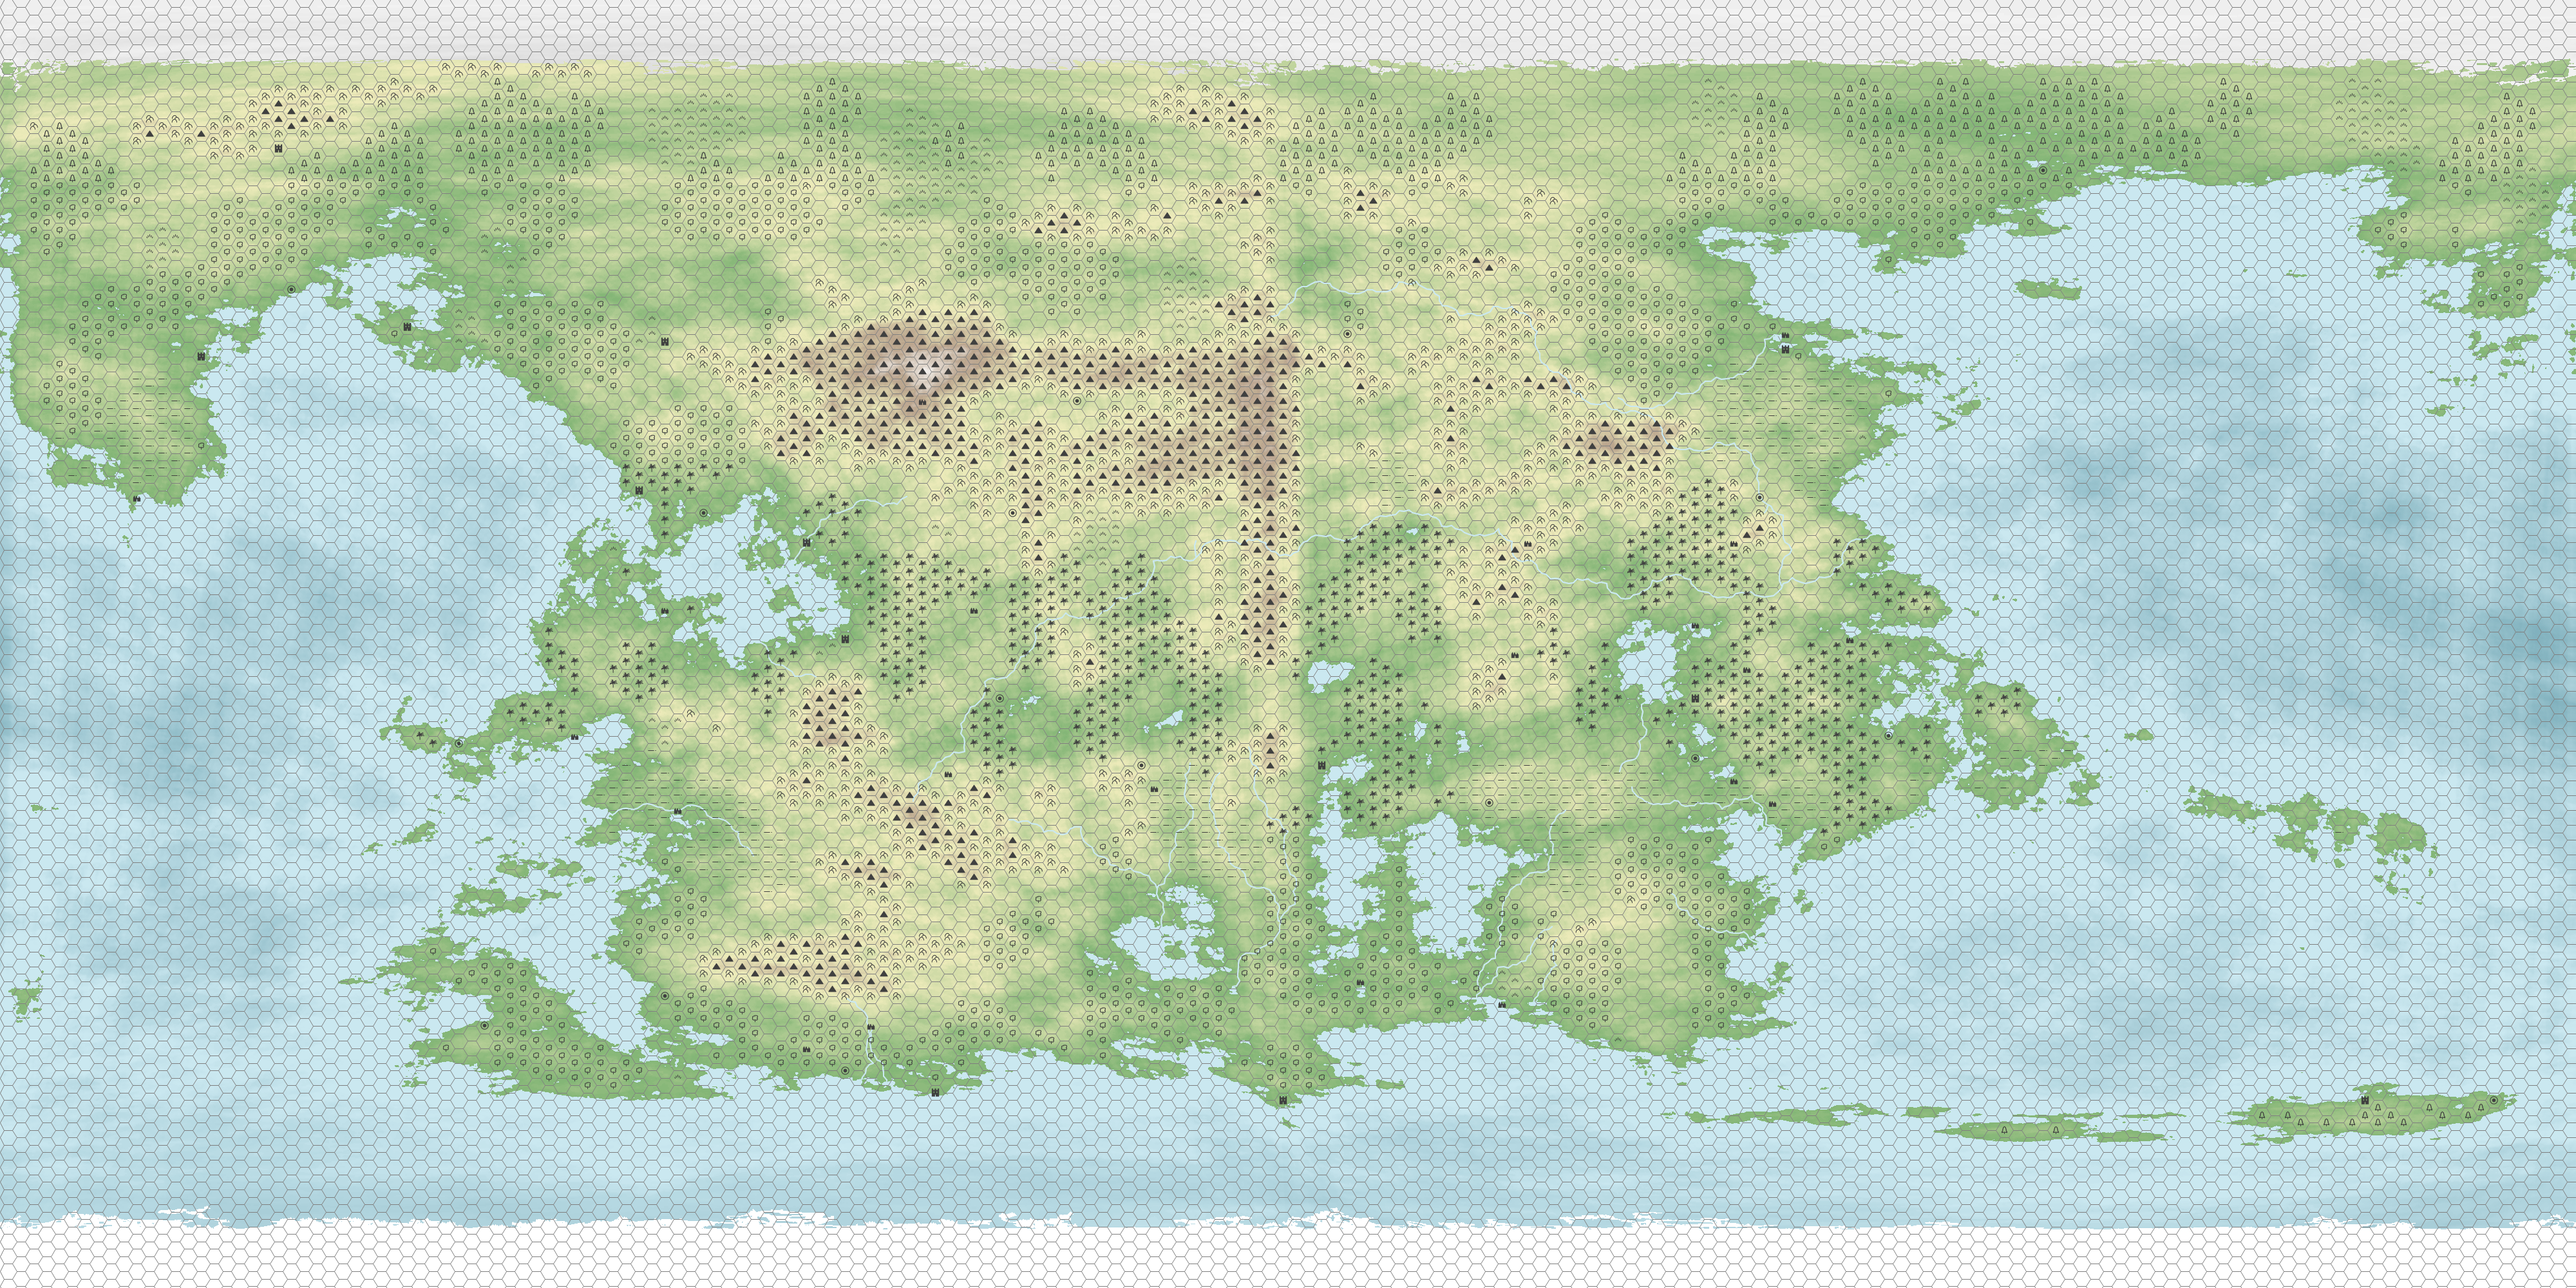
\includegraphics[width=\linewidth,keepaspectration=true]{img/maps/world-maps/Talaj.png}

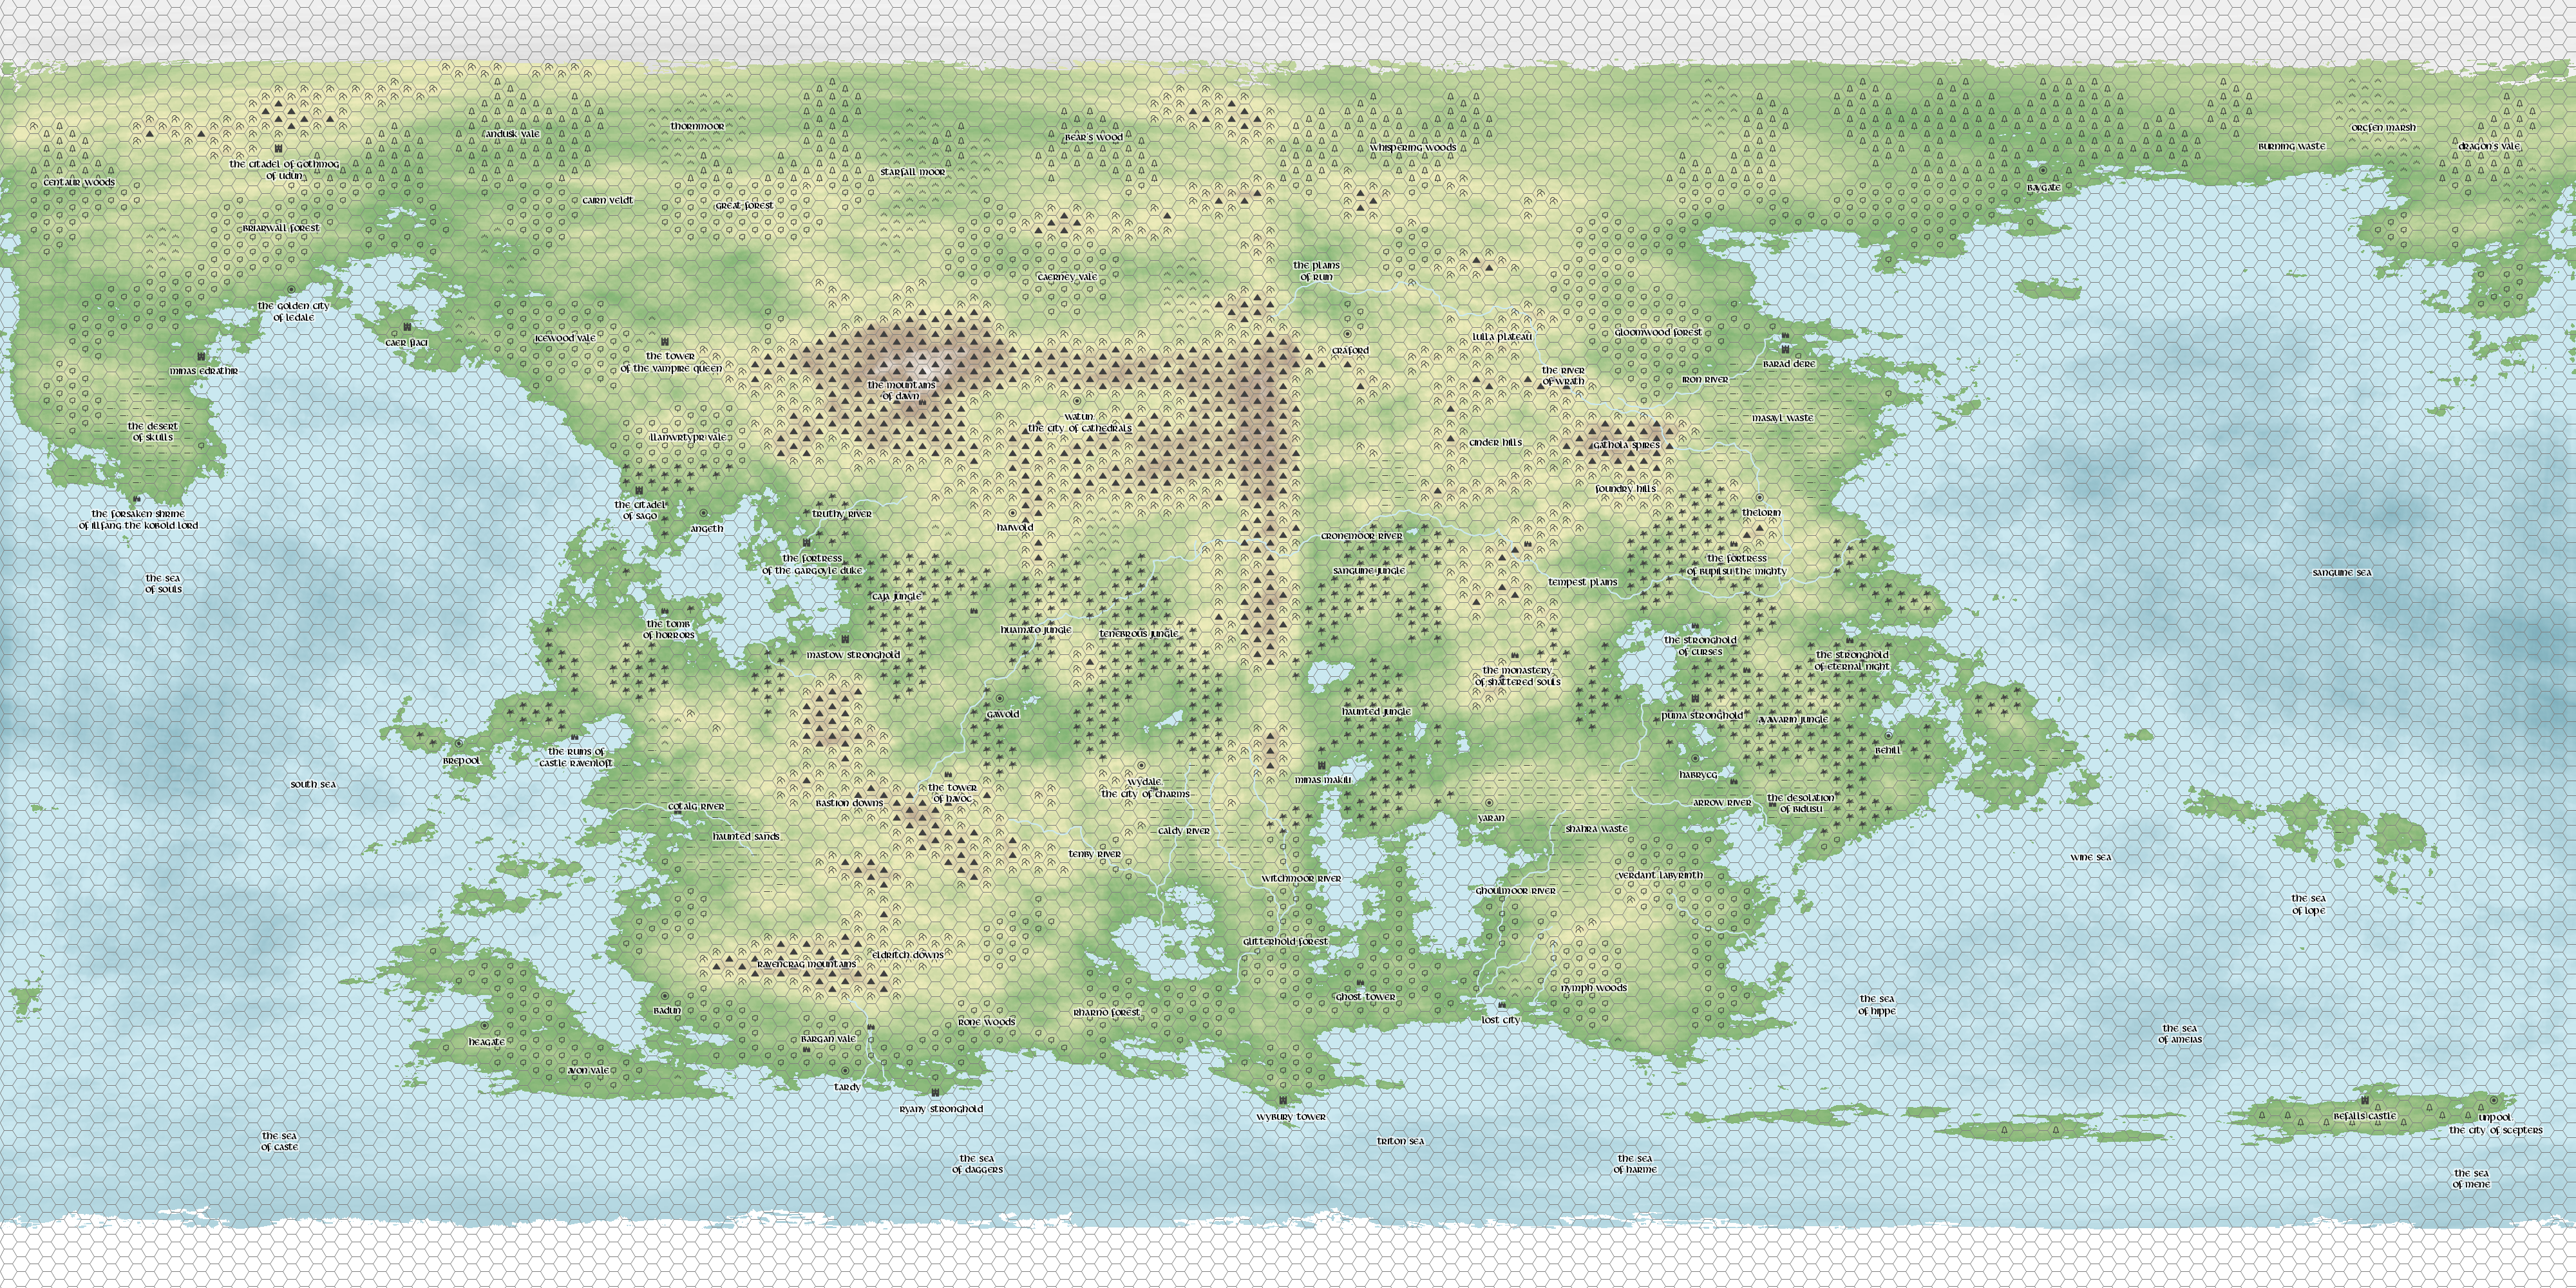
\includegraphics[width=\linewidth,keepaspectration=true]{img/maps/world-maps/Talaj2.png}


  \chapter{Setting}\label{ch:setting}

\chapter{Geography}\label{ch:geography}


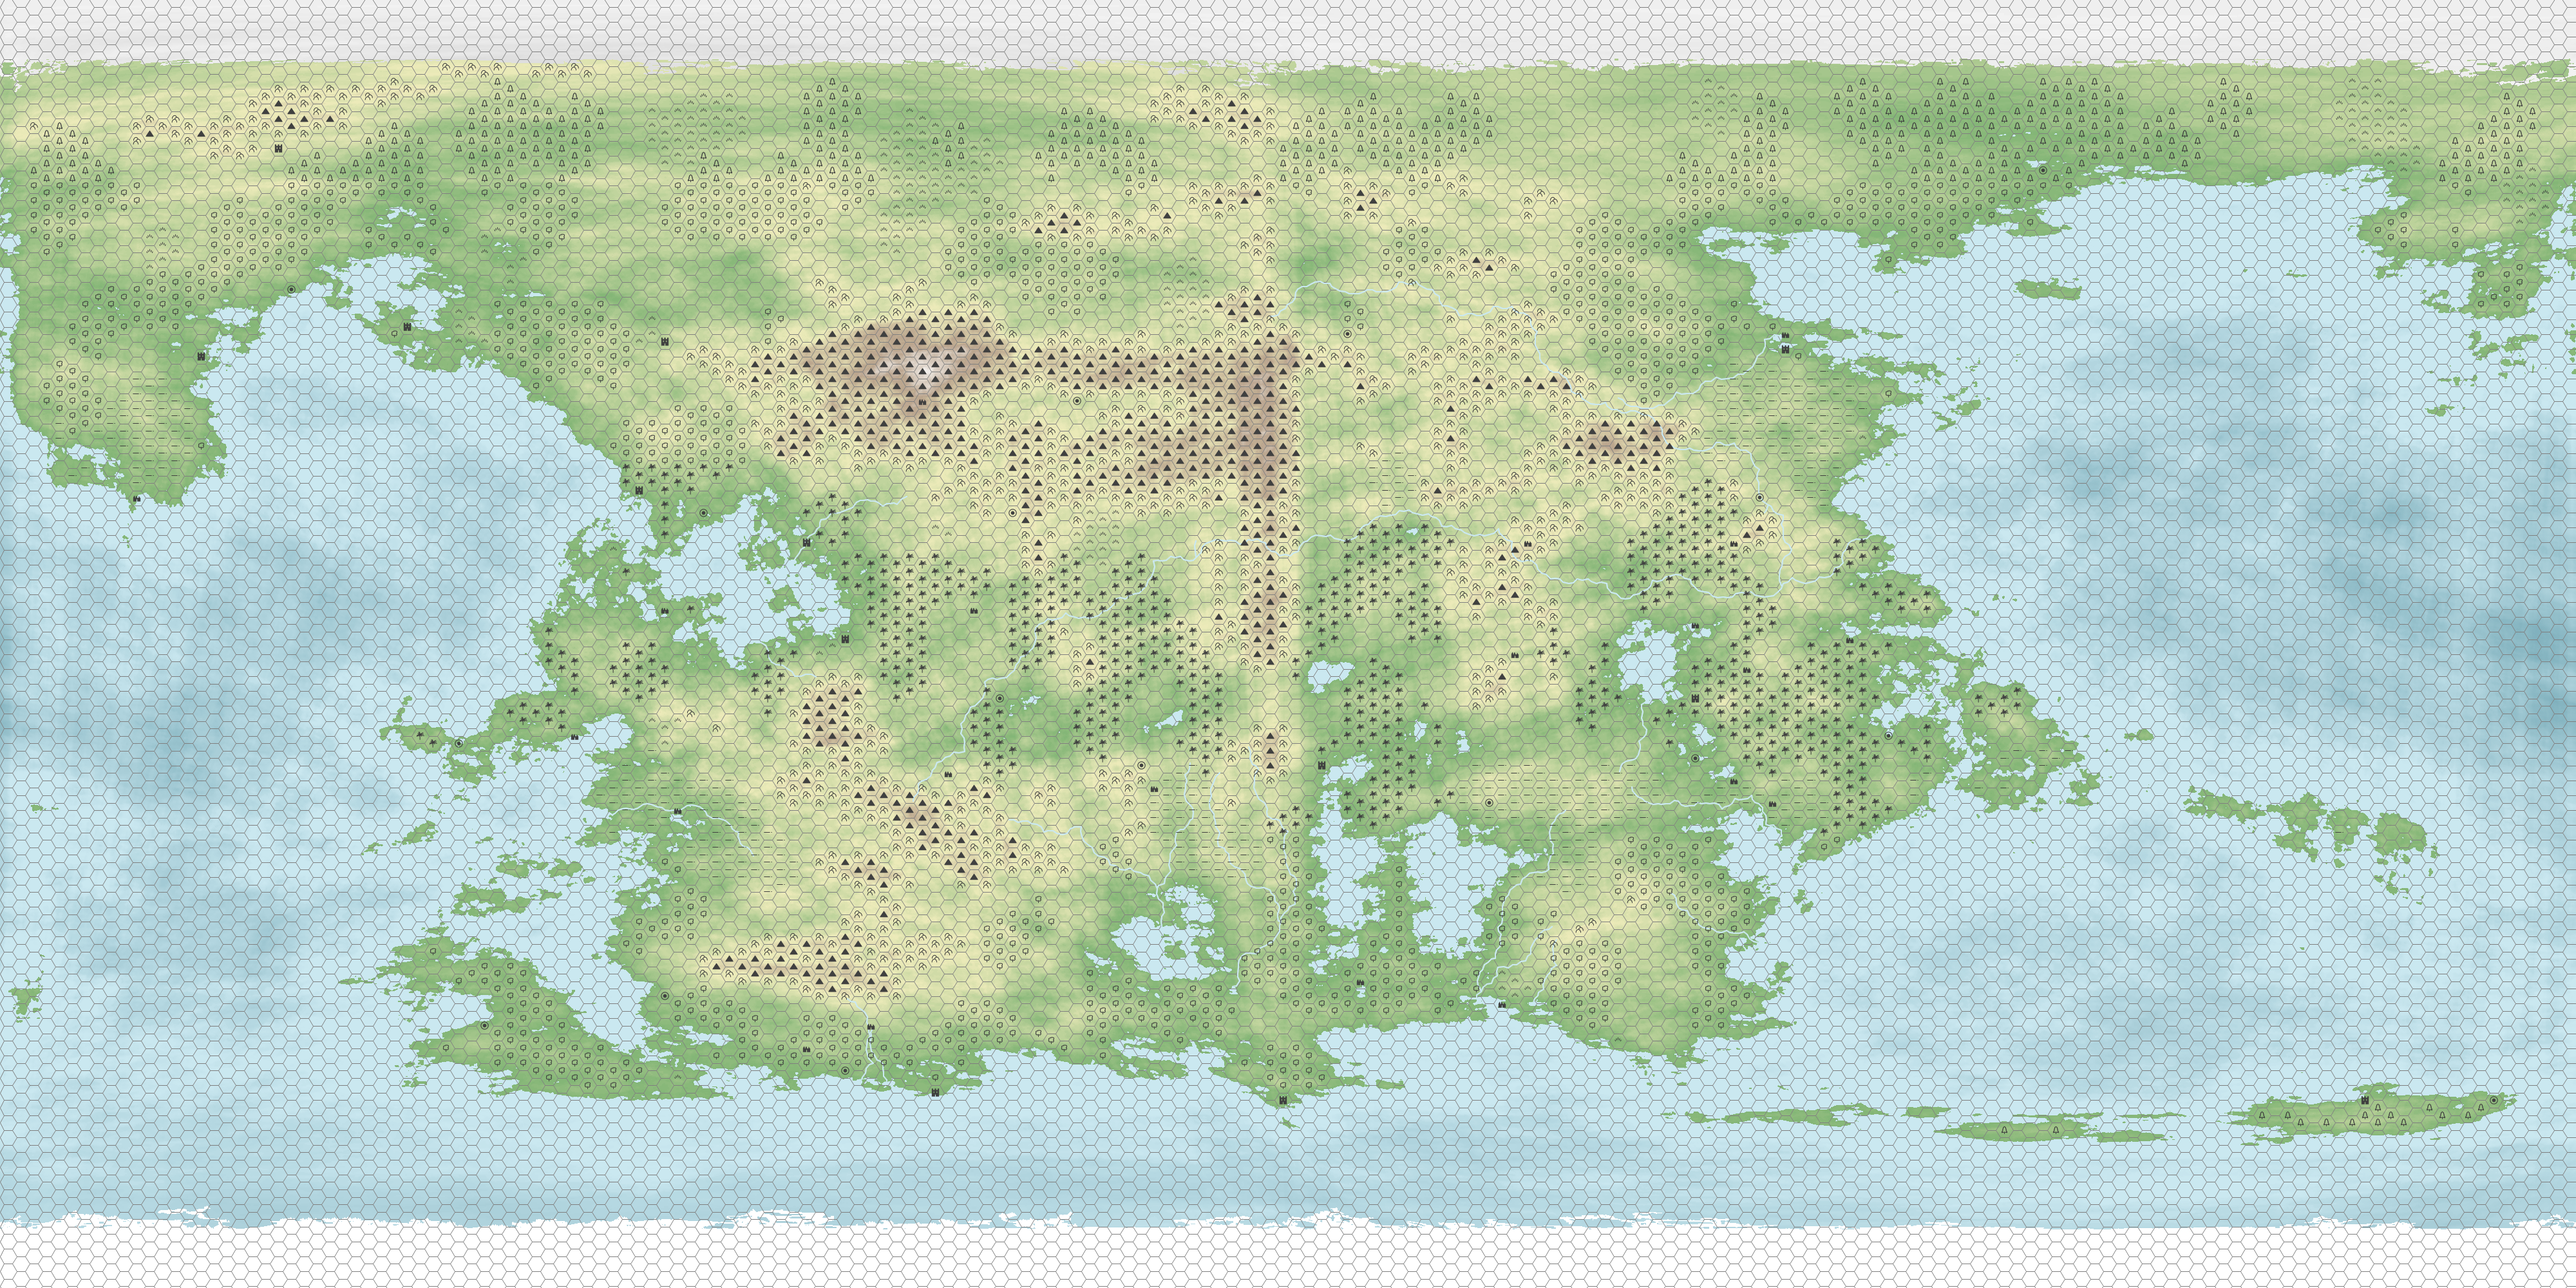
\includegraphics[width=\textwidth]{img/maps/world-maps/Talaj.png}

\input{setting/geography/the-empire.tex}
\input{setting/geography/the-northern-wylde.tex}
\input{setting/geography/the-southern-sea.tex}
\section{The Tribal Wastes}
\headeritem{Structure}{Fractured Clans}

Over the centuries, the beast tribes discovered in The Empire have been,
 if not slaughtered outright, driven east.
A partial misnomer, the Wastes are not a barren desert, but a lush grassland.
However, pockets of Gnolls, Goblins, Trolls, Orcs, Kobolds, Bullywugs, Lizardmen, and
 remnants of the once powerful Yuan-ti make travel into the Wastes lethal for almost
 all who enter it.

Aarakocra and Kenku tribes are also found in the Wastes.
These are often the only safe haven from an onslaught of violence that would befall those
 that must travel the Wastes.

\subsection{Boundary}
The Merlicut Gorge is maybe 1,500 feet across.
(Mississippi in the Quad Cities, give or take.)
Maybe short bridge to Arsenal Island with a redoubt, with the major bridge from there.



\subsection{Good monsters}

Axe Beak (CR: 1/4, Monster Manual p.317)

Blink Dog (CR: 1/4, Monster Manual p.318)

Blood Hawk (CR: 1/8, Monster Manual p.319)

Brown Bear (CR: 1, Monster Manual p.319)

Cockatrice (CR: 1/2, Monster Manual p.42)

Dire Wolf (CR: 1, Monster Manual p.321)

Elk (CR: 1/4, Monster Manual p.322)

Gnoll (CR: 1/2, Monster Manual p.163)

Goblin (CR: 1/4, Monster Manual p.166)

Harpy (CR: 1, Monster Manual p.181)

Hyena (CR: 0, Monster Manual p.331)

Orc (CR: 1/2, Monster Manual p.246)

Wolf (CR: 1/4, Monster Manual p.341)

Worg (CR: 1/2, Monster Manual p.341)

Yuan-ti Pureblood (CR: 1, Monster Manual p.310)



\section{The Western Horde}
\headeritem{Structure}{Hierarchical Magocracy}

Legion of Ayanum

Ruled by: The Silver Dragon, Ayanum.

Dragonborn ruling class, humans are a short-lived pestilence.



\input{setting/locations/locations}
\input{setting/lore/lore}

  \include{player-characters/player-characters}
  \include{characters/characters}
  \chapter{Plot}\label{ch:plot}

\input{story/00-preface/00-preface}
\input{story/01-celadirs-bastion/01-celadirs-bastion}

The Stone of Shomah

The Celadonian has heard of a powerful artifact called the Stone of Shomah located in a ruin
  not far into the Tribal Wastes.
He doesn't know what power it holds, but knows that the Yuan-ti fear it above all things.



\chapter{Important Things}
\section{Magic Items}
\subsection{The Bottom Dollar}
Magic coin of an arbitrary denomination.
When in a container with other coins, it will always be the last coin withdrawn.
A creature that remembers any identifying characteristic of the coin
  (that would distinguish it from another in the container) can withdraw the coin without emptying
  the container on a successful Intelligence saving throw (DC 15).

This coin is a favorite among diviners who would like to keep track of a particular person.
By paying for a good with a Bottom Dollar, or `tipping' them for some small service, the diviner
  can track the coin to track their mark by proxy.

\end{document}
